\documentclass{beamer}
\usepackage{tikz} %for mindmap
\usetikzlibrary{mindmap} %for mindmap
\usepackage{pgfpages}
\usepackage[backend=bibtex]{biblatex}
\usepackage{multicol}
\usepackage{textpos}
\setbeameroption{hide notes} % Only slides
%\setbeameroption{show only notes} % Only notes
%\setbeameroption{show notes on second screen=right} % Both
\bibliography{../../papers/references.bib}
\setbeamerfont{footnote}{size=\small}
%\AtEveryCitekey{\clearfield{title}}
\expandafter\def\expandafter\insertshorttitle\expandafter{%
   \insertshorttitle\hfill%
   \insertframenumber\,/\,\inserttotalframenumber}

%
% Choose how your presentation looks.
%
% For more themes, color themes and font themes, see:
% http://deic.uab.es/~iblanes/beamer_gallery/index_by_theme.html
%
\mode<presentation>
{
   \usetheme{Warsaw}      % or try Darmstadt, Madrid, Warsaw, ...
   \usecolortheme{default} % or try albatross, beaver, crane, ...
   \usefonttheme{default}  % or try serif, structurebold, ...
   \setbeamertemplate{navigation symbols}{}
%   \setbeamertemplate{caption}[numbered]
%   \setbeamertemplate{footline}[frame number]
   \usepackage{appendixnumberbeamer} %starts slide numbering over after \appendix
} 

\usepackage[english]{babel}
%\usepackage[utf8x]{inputenc} %Doesn't play well with biblatex
\usepackage{amssymb}
\usepackage{bm}
\usepackage{color}
\usepackage{graphicx}

\newcommand{\red}[1]{{\color{red}{#1}}}
\newcommand{\ket}[1]{\left| #1 \right>}
\newcommand{\bra}[1]{\left< #1 \right|}
\newcommand{\braket}[2]{\left< #1 | #2 \right>}
\newcommand{\ketbra}[2]{\left| #1 \right> \left< #2 \right|}
\newcommand{\expect}[1]{\left< #1 \right>}
\newcommand{\fpij}{f_p(r_{ij})}
\newcommand{\vpij}{v_p(r_{ij})}
\newcommand{\Opij}{\mathcal{O}_{ij}^p}
\newcommand{\fOpij}{\sum\limits_{i<j}\sum\limits_p \fpij\Opij}
\newcommand{\fqkl}{f_q(r_{kl})}
\newcommand{\Oqkl}{\mathcal{O}_{kl}^q}
\newcommand{\fOqkl}{\sum\limits_{k<l}\sum\limits_q \fqkl\Oqkl}
\newcommand{\fOqklip}{\sum\limits_{k<l,\mathrm{ip}}\sum\limits_q \fqkl\Oqkl}
\newcommand{\fOqklquad}{\sum_{\substack{k<l\\ij \ne kl}}\sum\limits_q \fqkl\Oqkl}
\newcommand{\f}[2]{f_{#1}(r_{#2})}
\renewcommand{\O}[2]{\mathcal{O}_{#2}^{#1}}
\newcommand{\fO}[2]{\sum\limits_{#1} f_{#1}(r_{#2})\mathcal{O}_{#2}^{#1}}
\newcommand{\R}{\mathbf{R}}
\newcommand{\dt}{\Delta\tau}
\newcommand{\ti}{\bm{\tau}_i}
\newcommand{\tj}{\bm{\tau}_j}
\newcommand{\si}{\bm{\sigma}_i}
\newcommand{\sj}{\bm{\sigma}_j}
\newcommand{\sfont}{6}
\newcommand{\sspace}{10.2}
\newcommand{\Oijp}{\mathcal{O}^p_{ij}}

\title[Improved Trial Wave Functions for Nuclear QMC]{Improved Trial Wave Functions for Nuclear Quantum Monte Carlo}
\author[Cody L. Petrie, cody.petrie@asu.edu]{Cody L. Petrie\\
Advisor: Kevin Schmidt}
\institute{Arizona State University \\ Tempe, AZ}
\date{}

\begin{document}

\begin{frame}
   \titlepage
%   \centering
%   \vspace{-1.0cm}
%   \small
%Collaborators: Stefano Gandolfi (LANL), Joe Carlson (LANL) \\~\\
%INT Program INT-18-2b Advances in Monte Carlo Techniques for Many-Body Quantum Systems \\
%July 30 - September 7, 2018
\end{frame}

\begin{frame}{Outline}
\begin{itemize}
   \item Quantum Monte Carlo methods
   \item Improved trial wave function
   \item Alpha formation in nearly neutron matter - preliminary
   \item Another Improved trial wave function - preliminary
   \item Future work/Conclusion
\end{itemize}
\end{frame}

\section{QMC Methods}
\begin{frame}{Quantum Monte Carlo}
\begin{itemize}
   \item \textbf{VMC:}
   \begin{equation*}
      E_V = \frac{\bra{\Psi_T}H\ket{\Psi_T}}{\braket{\Psi_T}{\Psi_T}} \ge E_0
   \end{equation*}
   \item \textbf{AFDMC:}
   \begin{equation*}
      \braket{\R_N}{\Psi_T(\tau)} = \int d\R_1 \ldots d\R_N \left[\prod\limits_{i=1}^N G(\R_i,\R_{i-1},\Delta\tau)\right] \braket{\R_0}{\Psi_T(0)}
   \end{equation*}
   \begin{equation*}
      G(\R',\R,\Delta\tau) = \bra{\R'}e^{-(H-E_0)\Delta\tau}\ket{\R}
   \end{equation*}
   \item $\Psi_T$ is calculated in practically every part of the calculation and plays an important role in guiding the propagation and diffusion of the calculation to the ground state.
\end{itemize}
\end{frame}

\section{Trial Wave Function}
\subsection{Spin-Dependent Correlations}
\begin{frame}{Slater Determinant}
\begin{itemize}
   \item Properties:
   \begin{itemize}
      \item Antisymmetric
      \item Cluster Decomposable \\ $\ket{A+B} = \ket{A}\ket{B}$
   \end{itemize}
   \begin{textblock*}{\textwidth}(4.5cm,-6.1cm) % {block width} (coords)
      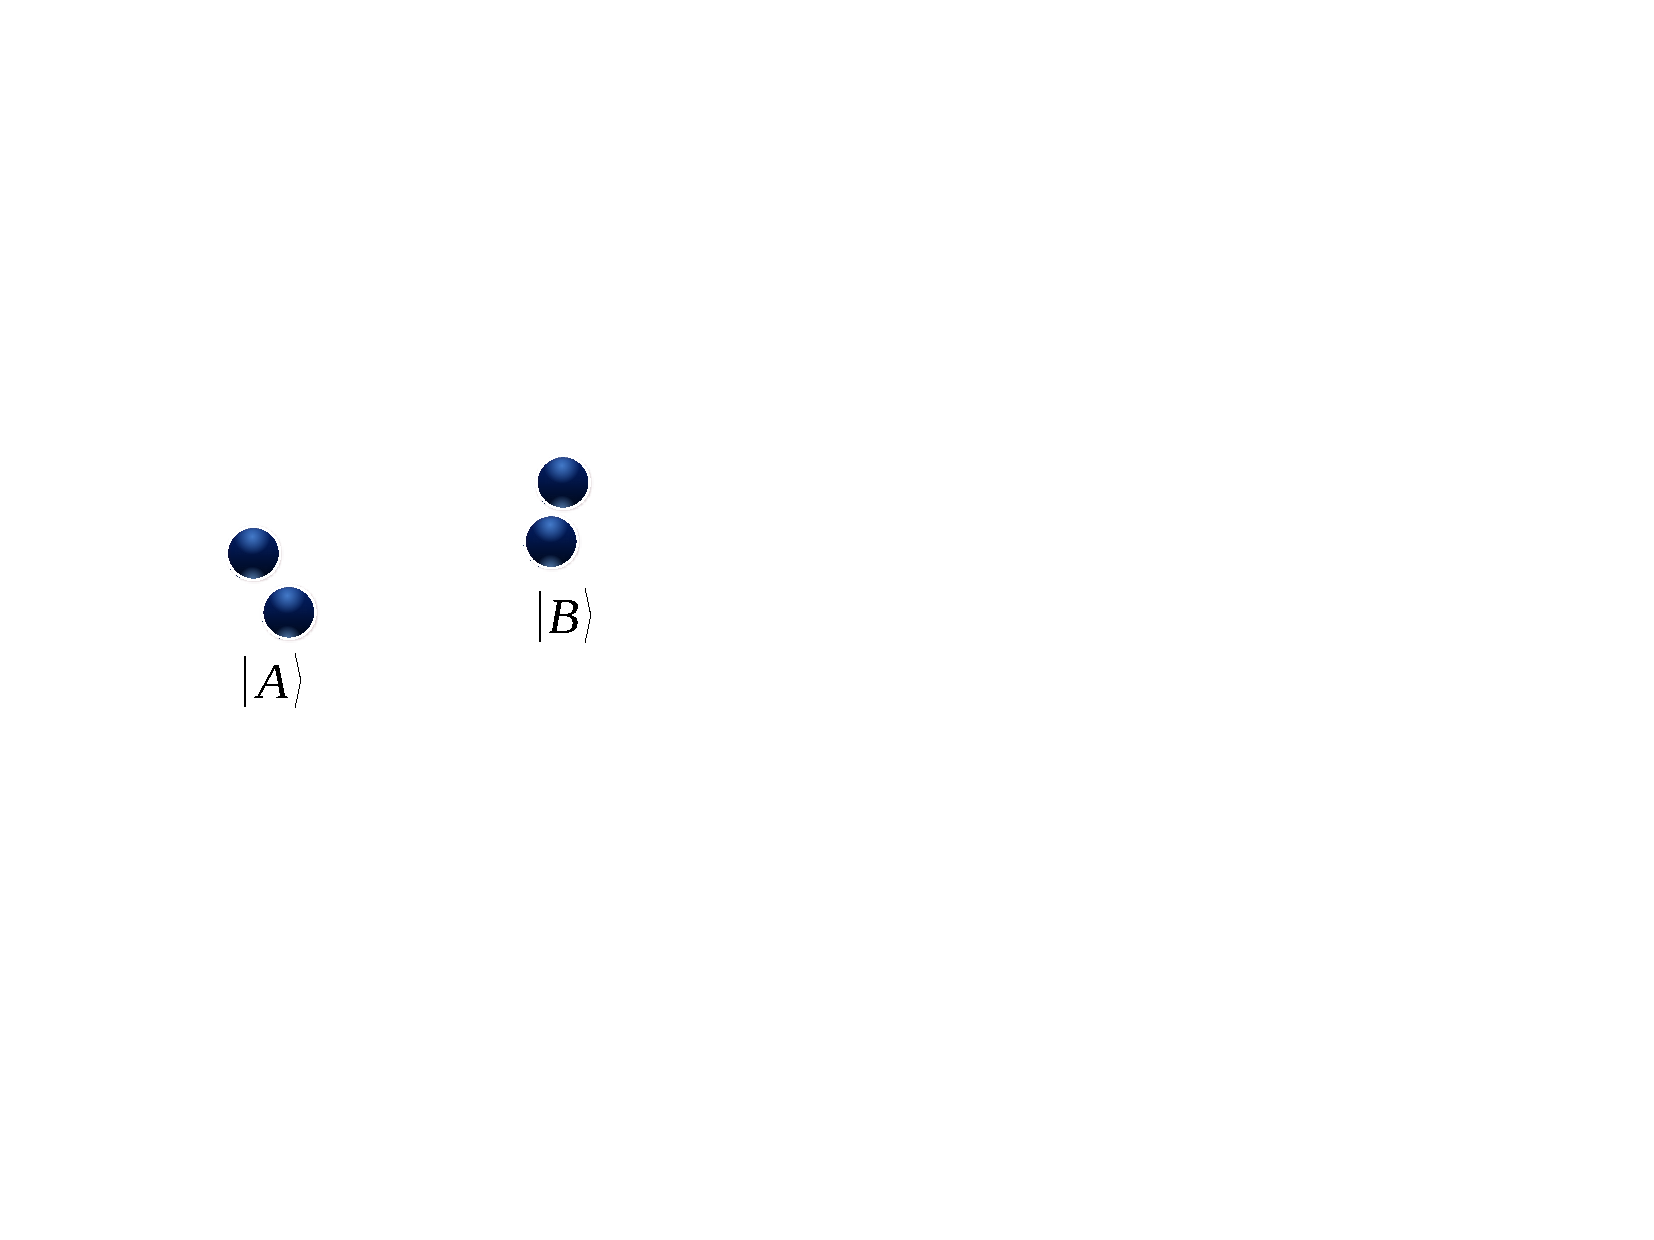
\includegraphics[width=14.6cm]{cluster.pdf}
   \end{textblock*}
   \item The simplest wave function for a many-fermion system obeying these properties is a Slater determinant where $\phi_i(\mathbf{r}_i,s_i)$ are single particle nucleon states.
   \begin{equation*}
      \psi_{T} = \braket{RS}{\phi}= \mathcal{A} \prod\limits_{i=1}^A \phi_i(\mathbf{r}_i,s_i) = \frac{1}{A!} \mathrm{det}~\phi_i(\mathbf{r}_i,s_i)
   \end{equation*}
   \item Short range correlations need to be put in by hand via Jastrow-like correlations.
   \begin{equation*}
      \ket{\psi_T} = \prod\limits_{i<j}f(r_{ij}) \ket{\phi}.
   \end{equation*}
\end{itemize}
\end{frame}

\begin{frame}{Spin Dependent Correlations}
\begin{itemize}
   \item Two spin dependent wave functions that obey these two properties are the exponentially correlated and symmetrized product wave functions, where $\Opij$ are the AV6 operators, $\si\cdot\sj$, $\ti\cdot\tj$,     $\si\cdot\sj \ti\cdot\tj$, $S_{ij}$ and $S_{ij} \ti\cdot\tj$, where $S_{ij}     = 3\si\cdot\hat{r}_{ij}\sj\cdot\hat{r}_{ij}-\si\cdot\sj$.
   \begin{equation*}
      \ket{\psi_T} = \left[\prod\limits_{i<j}f_c(r_{ij})\right] e^{\sum\limits_{i<j}\sum\limits_p\fpij\Opij} \ket{\phi}
   \end{equation*}
   \begin{equation*}
      \ket{\psi_T} = \left[\prod\limits_{i<j}f_c(r_{ij})\right] \mathcal{S}\prod\limits_{i<j}\left(1+\sum\limits_p\fpij\Opij\right) \ket{\phi}
   \end{equation*}
   \item These two wave functions are the same up to second order except for  commutator terms.
\end{itemize}
\end{frame}

\subsection{Quadratic Correlations}
\begin{frame}{Expand to Linear Correlations}
\begin{itemize}
   \item Because of the cost for larger systems in 2007 they only included Jastrow correlations.
   \begin{equation*}
      \ket{\psi_T} = \left[\prod\limits_{i<j}f_c(r_{ij})\right]\ket{\phi}
   \end{equation*}
   {\tiny S. Gandolfi et al. \textit{Phys. Rev. Lett.,} \textbf{99}, 022507, 2007.}
   \item By 2014 they added spin-isospin correlations to improve overlap with tensor. This is a truncated expansion of either full wave function from before.
   \begin{equation*}
      \ket{\psi_T} = \left[\prod\limits_{i<j}f_c(r_{ij})\right] \left(1+\sum\limits_{i<j}\sum\limits_p\fpij\Opij\right) \ket{\phi}
   \end{equation*}
   {\tiny S. Gandolfi et al. \textit{Phys. Rev. C.,} \textbf{90}, 061306(R), 2014.}
\end{itemize}
\end{frame}

\begin{frame}{Compare Jastrow to Jastrow+Linear}
\begin{figure}[h]
   \centering
   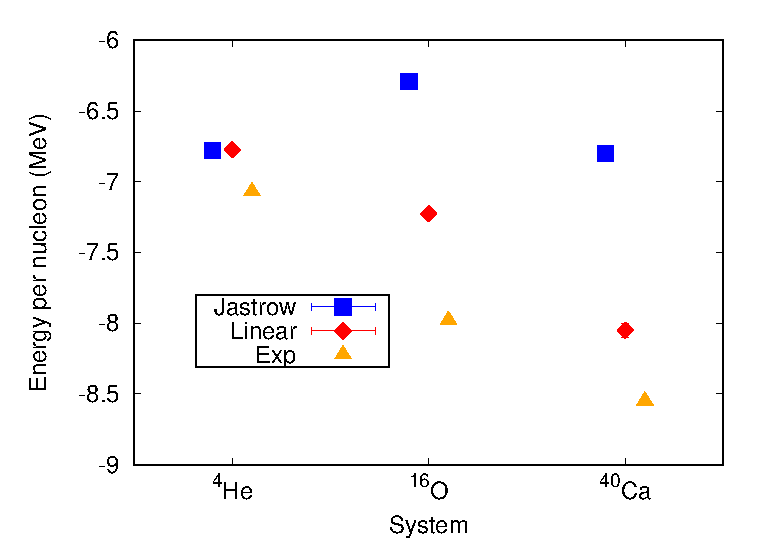
\includegraphics[width=0.85\textwidth]{energy_jaslin.eps}
\end{figure}
\vspace{-0.5cm}
{\tiny Data taken from each paper respectively.}
\end{frame}

\begin{frame}{Symmetrized Product Wave Function}
\begin{itemize}
   \item The logical next step was to keep more terms in the expansion.
   \begin{equation*}
   \begin{split}
      \ket{\psi_T} = \Bigg[\prod\limits_{i<j}&f_c(r_{ij})\Bigg] \Bigg[1+\fOpij \\
      & + \frac{1}{2}\fOpij\fOqklquad \Bigg] \ket{\phi}
   \end{split}
   \end{equation*}
\end{itemize}
\begin{figure}[h]
   \centering
   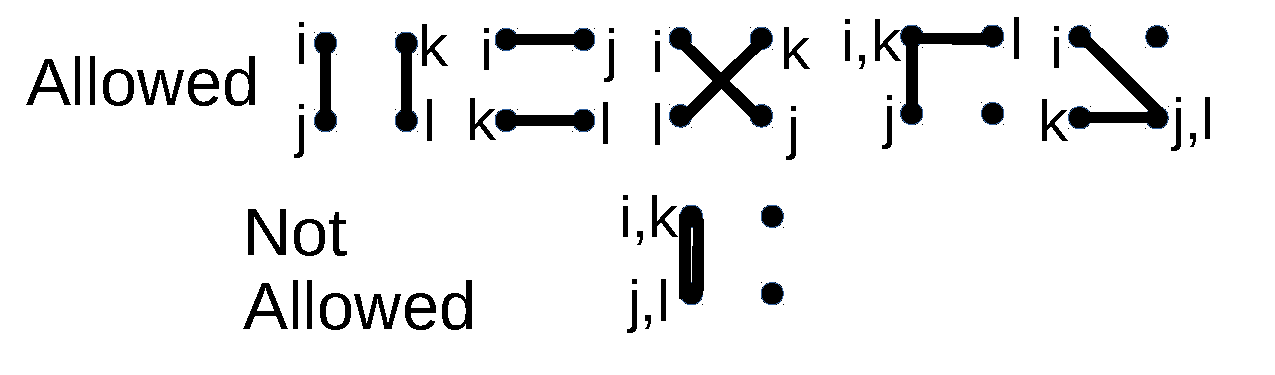
\includegraphics[width=1.0\textwidth]{pairing_fullquad.pdf}
\end{figure}
\end{frame}

\begin{frame}{Independent Pair Quadratic Correlations}
\begin{itemize}
   \item Or it can be expanded to get independent pair quadratic terms
   \begin{equation*}
   \begin{split}
      \ket{\psi_T} = \Bigg[\prod\limits_{i<j}&f_c(r_{ij})\Bigg] \Bigg[1+\fOpij \\
      & + \fOpij\fOqklip \Bigg] \ket{\phi}
   \end{split}
   \end{equation*}
\end{itemize}
\begin{figure}[h]
   \centering
   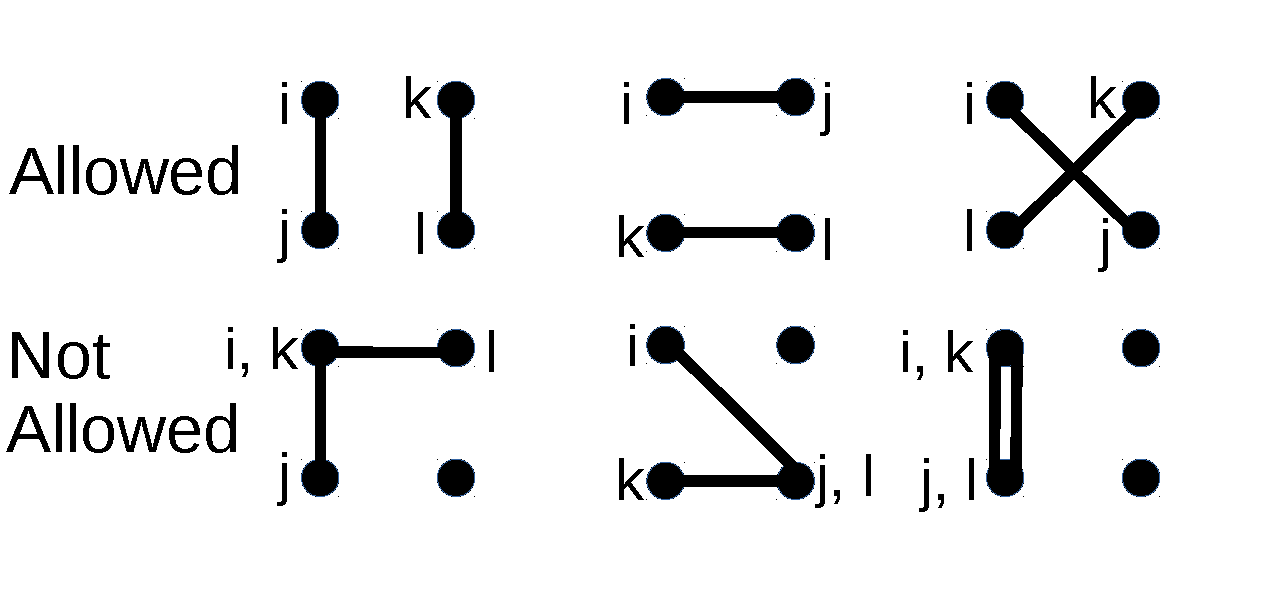
\includegraphics[width=0.7\textwidth]{pairing.pdf}
\end{figure}
\end{frame}

\begin{frame}{Results}
\begin{textblock*}{\textwidth}(0.0cm,-0.6cm) % {block width} (coords)
\begin{figure}[h]
   \centering
   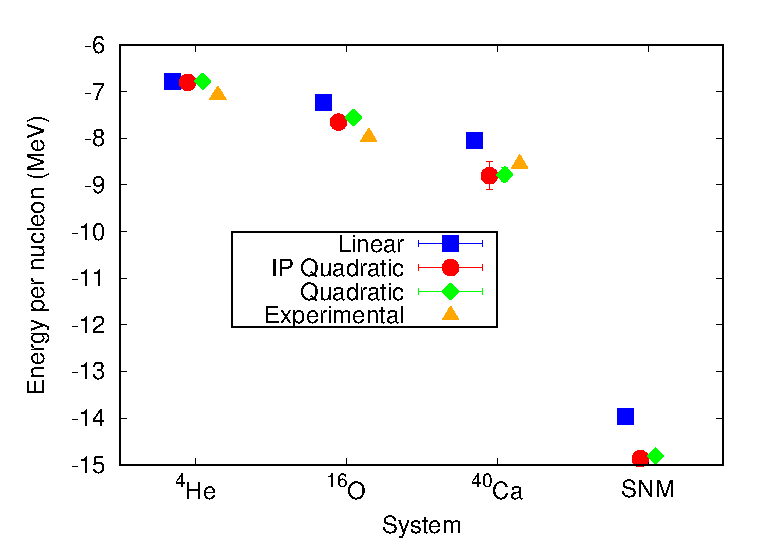
\includegraphics[width=0.6\textwidth]{energy.eps}
\end{figure}
\end{textblock*}
~\\~\\~\\~\\~\\~\\~\\~\\
\tiny
\begin{table}[htb]
\centering
\caption[]{Energy (*per nucleon) in MeV}
\begin{tabular}{ccccc}
\hline\hline
System & Linear & IP Quadratic & Quadratic & Experimental\\
\hline
%${}^{4}${He}   & -27.14(4) & -27.22(3)    & -27.11(3)    & -28.295   \\
%${}^{16}${O}   & -115.7(9) & -121.5(1.5)  & -120.0(1.4)  & -127.62   \\
%${}^{40}${Ca}  & -324(3)   & -347(8)      & -349(5)      & -342.1    \\
%SNM*           & -13.92(6) & -14.80(7)    & -14.70(11)   &           \\
${}^{4}${He}   & -27.14(4) & -27.19(3)    & -27.11(3)    & -28.296   \\
${}^{16}${O}   & -115.7(9) & -122.4(1.5)  & -120.8(1.3)  & -127.62   \\
${}^{40}${Ca}  & -322(3)   & -350(10)     & -351(6)      & -342.1    \\
SNM*           & -13.97(3) & -14.87(4)    & -14.81(3)    &           \\
\hline\hline
\end{tabular}
\label{tab:psi2}
\end{table}
{\tiny D. Lonardoni et al. \textit{Phys. Rev. C.,} \textbf{97}, 044318, 2018.}
\end{frame}

\begin{frame}{Quadratic Correlation Cost}
\begin{figure}[h]
   \centering
   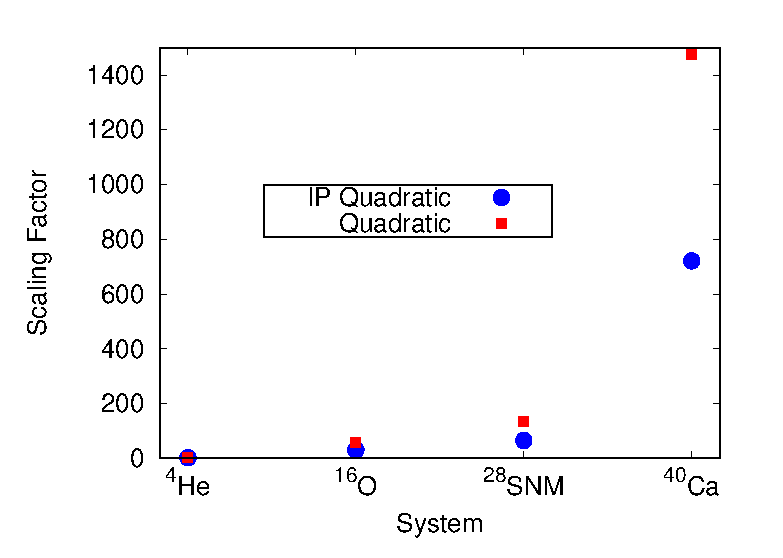
\includegraphics[width=0.65\textwidth]{scaling.eps}
\end{figure}
\vspace{-0.2cm}
\begin{table}[h!]
   \centering
   \begin{tabular}{ccccc}
      \hline \hline
       & $^{4}$He & $^{16}$O & SNM(28) & $^{40}$Ca \\
      \hline
      IP Quadratic & 1.73 & 30.7 & 64.8 & 720.9 \\
      Quadratic & 2.00 & 58.8 & 133.6 & 1473.9 \\
      \hline \hline
   \end{tabular}
\end{table}
\end{frame}

\subsection{Application to NS}
\begin{frame}{Neutron Stars}
\begin{figure}[h]
   \centering
   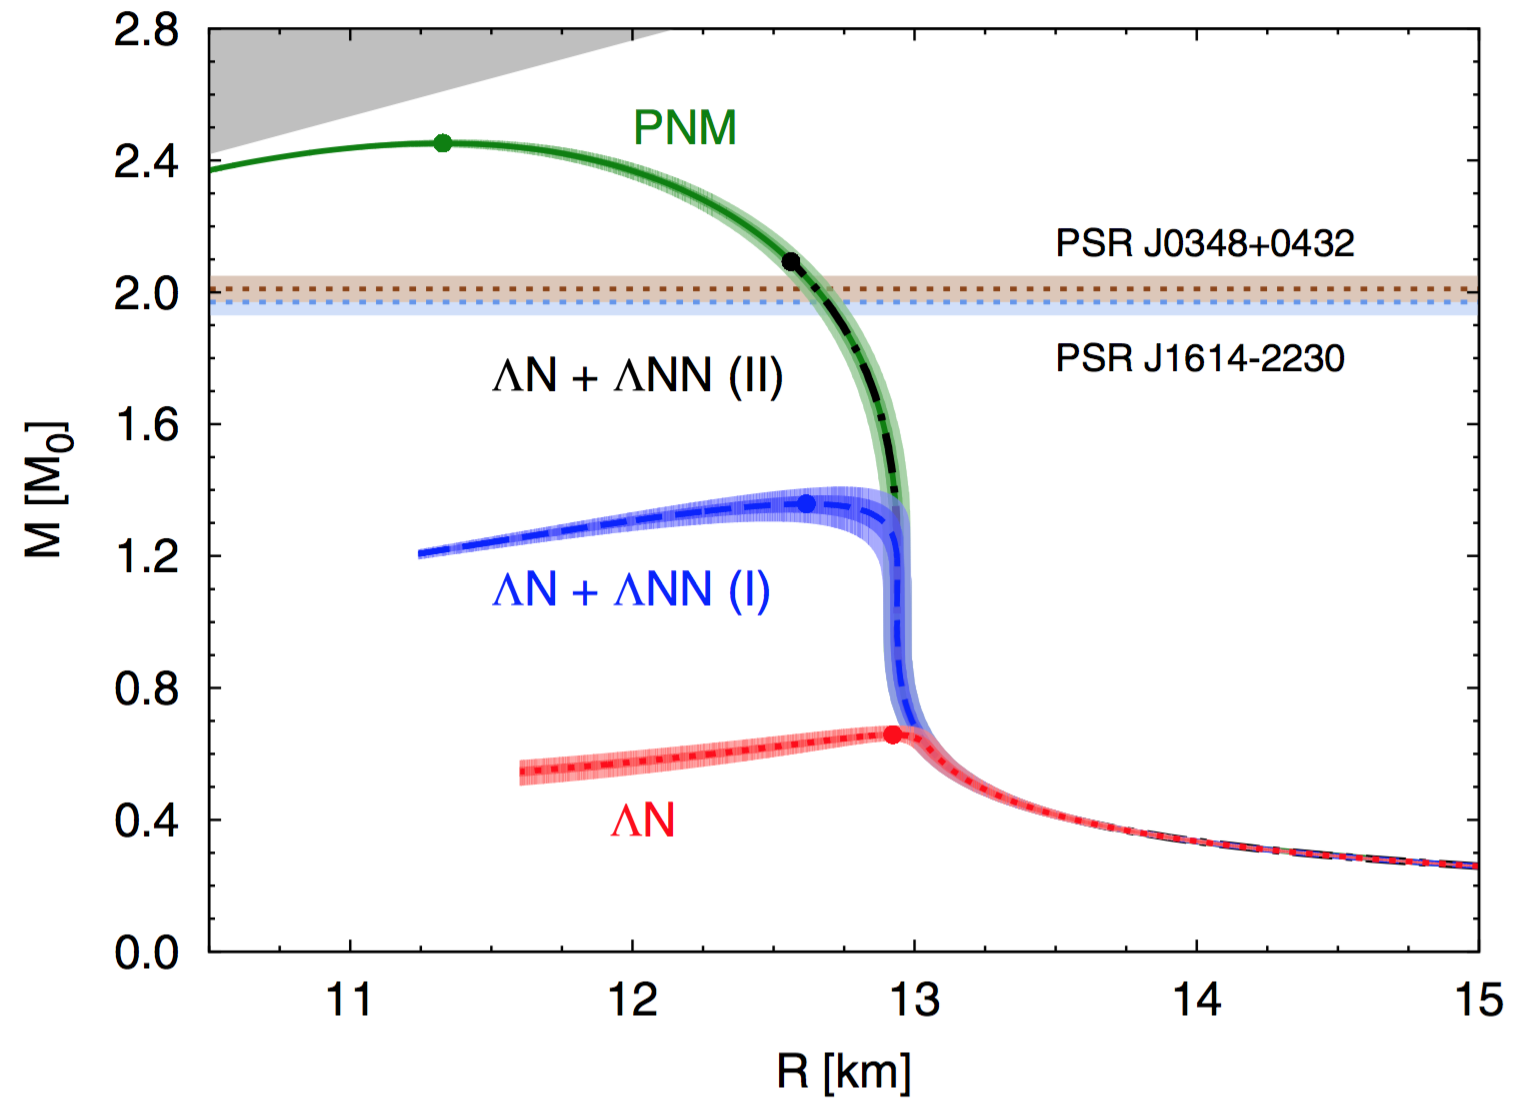
\includegraphics[width=0.7\textwidth]{mr.png}
\end{figure}
\vspace{-0.5cm}
{\tiny Diego Lonardoni et al. \textit{Phys. Rev. Lett.,} \textbf{114}, 092301, 2015.}
\end{frame}

\begin{frame}{Neutron Stars - Preliminary}
\begin{itemize}
   \item Use new wave function to study $\alpha$ formation in the inner crust of neutron stars.
   \begin{equation*}
      E_\alpha = E_\text{Nn+2p} - E_\text{(N-2)n}
   \end{equation*}
\end{itemize}
\vspace{-0.5cm}
\begin{figure}[h]
   \centering
   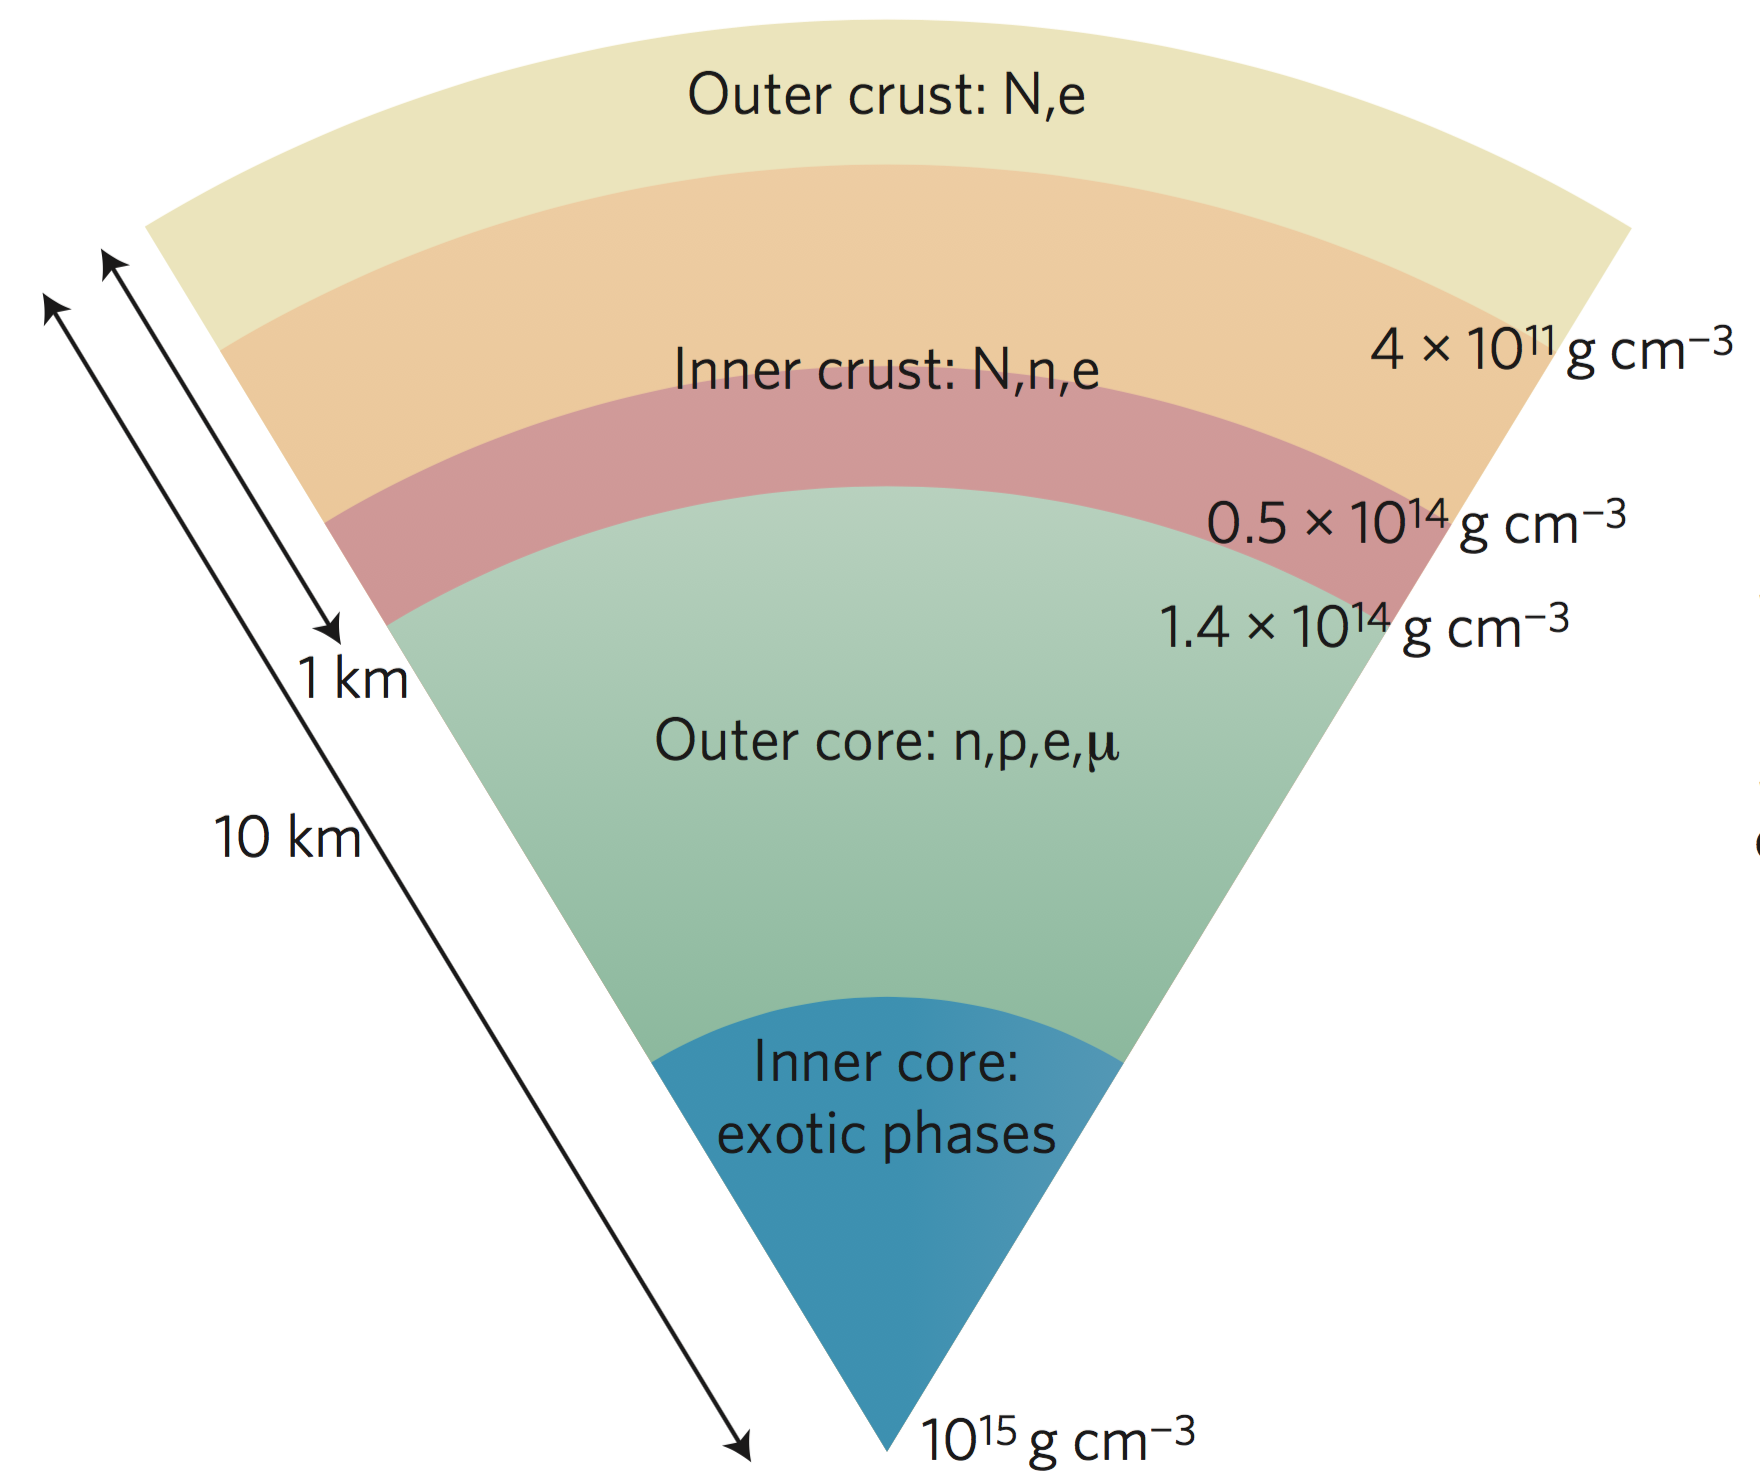
\includegraphics[width=0.5\textwidth]{neutronstar.png}
\end{figure}
{\tiny W. Newton {\it Nature Physics} {\bf 9}, 396-397 (2013)}
%\begin{textblock*}{\textwidth}(8.1cm,-4.6cm) % {block width} (coords)
\begin{textblock*}{\textwidth}(8.1cm,-4.4cm) % {block width} (coords)
   \tiny $\approx$ 0.00024 fm$^{-3}$
\end{textblock*}
%\begin{textblock*}{\textwidth}(7.8cm,-4.1cm) % {block width} (coords)
\begin{textblock*}{\textwidth}(7.8cm,-3.9cm) % {block width} (coords)
   \tiny $\approx$ 0.030 fm$^{-3}$
\end{textblock*}
%\begin{textblock*}{\textwidth}(7.6cm,-3.8cm) % {block width} (coords)
\begin{textblock*}{\textwidth}(7.6cm,-3.6cm) % {block width} (coords)
   \tiny $\approx$ 0.084 fm$^{-3}$
\end{textblock*}
%\begin{textblock*}{\textwidth}(6.4cm,-1.3cm) % {block width} (coords)
\begin{textblock*}{\textwidth}(6.4cm,-1.1cm) % {block width} (coords)
   \tiny $\approx$ 0.60 fm$^{-3}$
\end{textblock*}
\end{frame}

\begin{frame}{\large Alpha Particle Clustering in Mostly Neutron Matter - Preliminary}
\begin{itemize}
   \item If alpha particles form in nearly neutron matter then we should be able to estimate their energy by
   \begin{equation*}
      E_\alpha = E_\text{14n+2p} - E_\text{12n}
   \end{equation*}
   \vspace{-0.25cm}
   \begin{columns}
   \begin{column}{0.6\textwidth}
   \begin{figure}[h]
      \centering
      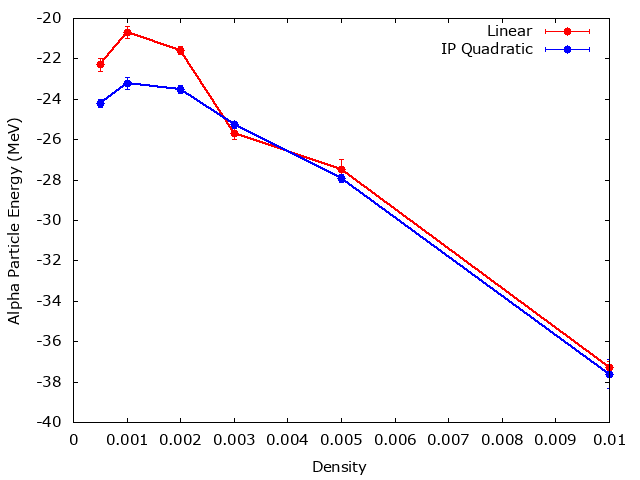
\includegraphics[width=\textwidth]{alpha.png}
   \end{figure}
   \end{column}
   \hspace{-0.6cm}
   \begin{column}{0.4\textwidth}
   \begin{table}[h!]
      \footnotesize
      \centering
      \caption{Alpha energy in MeV}
      \begin{tabular}{ccc}
         \hline \hline
         $\rho$ (fm$^{-3}$) & lin & ip \\
         \hline
         0.0005& -22.3(3)  & -24.2(2)  \\  
         0.001 & -20.7(3)  & -23.2(3)  \\  
         0.002 & -21.6(2)  & -23.5(3)  \\  
         0.003 & -25.7(3)  & -25.26(18)\\
         0.005 & -27.5(5)  & -27.9(2)  \\  
         0.01  & -37.3(3)  & -37.6(7)  \\  
         \hline \hline
      \end{tabular}
   \end{table}
   \end{column}
   \hspace{0.6cm}
   \end{columns}
\end{itemize}
\end{frame}

\begin{frame}{Pair Correlation Function - Preliminary}
\vspace{-0.1cm}
\begin{equation*}
   g_{pp}(r) = \frac{1}{4\pi r^2} \bra{\Psi}\sum\limits_{i<j}\hat{p}_i\hat{p}_j\delta(r-r_{ij})\ket{\Psi}
\end{equation*}
\vspace{-0.4cm}
\begin{figure}[h]
   \centering
   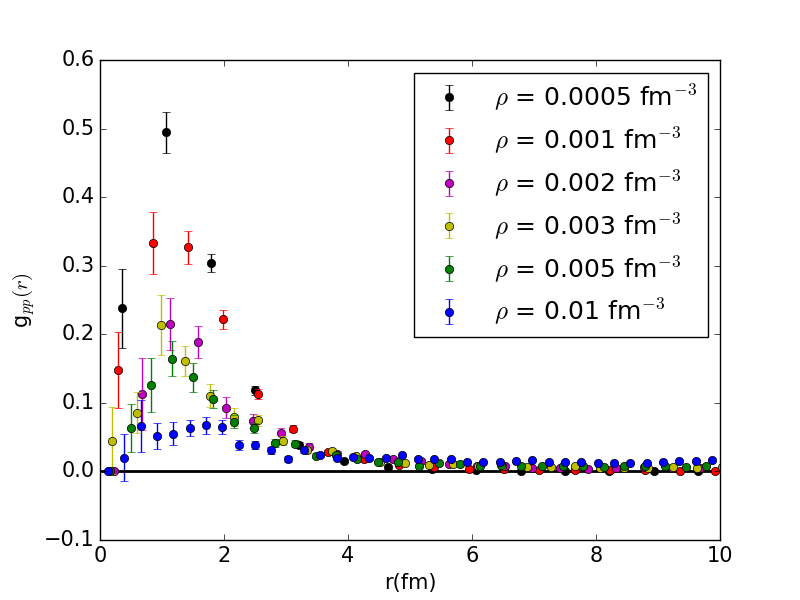
\includegraphics[width=0.70\textwidth]{gpp.png}
\end{figure}
\end{frame}

\subsection{Exponential Correlations}
\begin{frame}{Exponential Correlations - Preliminary}
\begin{itemize}
   \item The quadratic correlations improved the trial wave function, but with a large computational cost. Can we do better with the exponential correlations?
   \begin{equation*}
      \ket{\psi_T} = \left[\prod\limits_{i<j}f_c(r_{ij})\right] e^{\sum\limits_{i<j}\sum\limits_p\fpij\Opij} \ket{\phi}
   \end{equation*}
   \item We don't know how to calculate the exponential of two-body operators. But we have already tackled this exact problem with the spin sampling in AFDMC by using the Hubbard-Stratanovich transformation.
\begin{equation*}
      e^{-\frac{1}{2}\lambda O_i^2} = \frac{1}{\sqrt{2\pi}} \int dx e^{-\frac{x^2}{2} + \sqrt{-\lambda}xO_i}
   \end{equation*}
\end{itemize}
\end{frame}

\begin{frame}{Exponential Correlations - Preliminary}
\begin{itemize}
   \item Following the same procedure used in AFDMC spin sampling we can write the exponential correlations as
   \begin{equation*}
      \exp\left(\sum\limits_{i<j,p}f_p(r_{ij})\Oijp\right) = \exp\left(\frac{1}{2}\sum\limits_{n=1}^{15A} \left(O_{n}\right)^2 \lambda_n^{\sigma}\right),
%         &= \left[\prod\limits_{i<j}f_c(r_{ij})\right] e^{\frac{1}{2}\sum\limits_{n=1}^{3A} \left(O_{n}^{\sigma}\right)^2 \lambda_n^{\sigma}
%         + \frac{1}{2}\sum\limits_{\alpha=1}^{3}\sum\limits_{n=1}^{3A} \left(O_{n\alpha}^{\sigma\tau}\right)^2 \lambda_n^{\sigma\tau}
%         + \frac{1}{2}\sum\limits_{\alpha=1}^{3}\sum\limits_{n=1}^{A} \left(O_{n\alpha}^{\tau}\right)^2 \lambda_n^{\tau}} \ket{\phi}
   \end{equation*}
   where the $3A$ $O_{n}^{\sigma}$, $9A$ $O_{n\alpha}^{\sigma\tau}$, and $3A$ $O_{n\alpha}^{\tau}$ single particle operators are
   \begin{equation*}
   \begin{split}
      O_{n}^{\sigma} &= \sum\limits_{j,\beta} \sigma_{j,\beta}\psi_{n,j,\beta}^{\sigma} \\
      O_{n\alpha}^{\sigma\tau} &= \sum\limits_{j,\beta} \tau_{j,\alpha}\sigma_{j,\beta}\psi_{n,j,\beta}^{\sigma\tau} \\
      O_{n\alpha}^{\tau} &= \sum\limits_{j} \tau_{j,\alpha}\psi_{n,j}^{\tau}.
   \end{split}
   \end{equation*}
\end{itemize}
\end{frame}

\begin{frame}{Exponential Correlations - Preliminary}
\begin{itemize}
   \item Using the Hubbard-Stratanovich transformation this can then be written as
   \begin{equation}
      \exp\left(\frac{1}{2}\sum\limits_{n=1}^{15A} \left(O_{n}\right)^2 \lambda_n^{\sigma}\right) = \prod\limits_{n=1}^{15A} \frac{1}{\sqrt{2\pi}}\int dx_n e^{-x_n^2/2}e^{\sqrt{\lambda_n}x_nO_n},
   \end{equation}
   and the auxiliary fields can be sampled to be
   \begin{equation}
      \Psi_T(R,S) = \bra{RS}\prod\limits_{n=1}^{15A} \frac{1}{N} \sum\limits_{\{x_n\}}^N\frac{1}{\sqrt{2\pi}}e^{\sqrt{\lambda_n}x_nO_n}\ket{\Phi}.
   \end{equation}
\end{itemize}
\end{frame}

\begin{frame}{Exponential Correlations - Preliminary}
\begin{itemize}
   \item Problems with statistical errors related to the sampling.
   \item Calculating the potential energy with exponential correlations and the rest with linear correlations.
   \vspace{-0.2cm}
   \begin{columns}
   \begin{column}{0.5\textwidth}
   \begin{figure}[h]
      \centering
      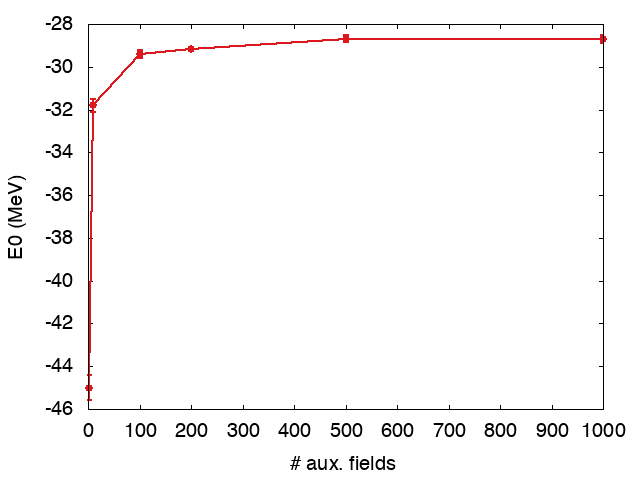
\includegraphics[width=\textwidth]{expplot.png}
   \end{figure}
   \end{column}
   \begin{column}{0.5\textwidth}
   \begin{table}[h!]
      \centering
      \caption{$^{4}$He energy with exp correlations. E$_\text{linear}$=-26.48(9) MeV.}
      \begin{tabular}{cc}
         \hline \hline
         \# fields & E (MeV) \\
         \hline
         1     & -45.0(6)  \\
         10    & -31.8(3)  \\
         100   & -29.4(2)  \\
         200   & -29.15(8) \\
         500   & -28.68(18)\\
         1000  & -28.7(2)  \\
         \hline \hline
      \end{tabular}
   \end{table}
   \end{column}
   \end{columns}
   \item Currently looking into this problem.
\end{itemize}
\end{frame}

\section{Conclusion}
\begin{frame}{Future Work}
\begin{itemize}
   \item Neutron star equation of state
   \begin{itemize}
      \item Using $\chi$EFT interaction
      \item Understanding the hyperon problem
   \end{itemize}
   \item Understand what is happening at higher nuclear densities
   \item Other interesting projects that push our understanding and application of nuclear physics
\end{itemize}
\end{frame}

\begin{frame}{Summary/Conclusion}
\begin{itemize}
   \item We have improved the previously used two-body spin-isospin correlations.
   \item The improved trial wave functions appear to make a significant difference in the energy of the calculations, but currently cost too much to use for large systems.
   \item We have shown that our calculation can see what are probably alpha particles forming in mostly neutron matter around the density of neutron star crusts. These calculations appear to be even better when improved correlations are used.
\end{itemize}
\end{frame}

%\note[itemize]{
%   \item test1
%   \item test2
%}

\begin{frame}{Thanks}
Advisor: Kevin Schmidt (ASU) \\
Collaborators: Stefano Gandolfi (LANL) and Joe Carlson (LANL)
\\~\\
\begin{figure}[h]
   \centering
   
\includegraphics[width=0.30\textwidth]{asu_university_vert_rgb_maroongold_150.png}
   
\includegraphics[width=0.36\textwidth]{xsede-full-color.jpg}
   
\includegraphics[width=0.30\textwidth]{NSF_4-Color_bitmap_Logo.png}
\end{figure}
\end{frame}

\iffalse
\appendix
\begin{frame}{Variational Monte Carlo - Implementation}
\begin{enumerate}
   \item Generate N configurations (walkers) distributed randomly.
   \item Loop over each walker and do the following
   \begin{enumerate}
      \setlength\itemsep{0.2em}
      \item Calculate $P(\R) = \left|\braket{\Psi_T}{\R}\right|^2$.
      \item Propose a move $\R' = \R + \Delta\xi$, where $\xi$ could be a vector of random variables from a Gaussian.
      \item Calculate $P(\R') = \left|\braket{\Psi_T}{\R'}\right|^2$.
      \item Calculate the probability of acceptance $A=\mathrm{min}\left(1,\frac{P(\R')}{P(\R)}\right)$.
      \item If accepted then $\R \rightarrow \R'$, else the next position in the Markov Chain for that walker is the same as the last, namely $\R$.
   \end{enumerate}
   \item Calculate observables and repeat steps 2 until energy is minimized or uncertainties are low enough.
\end{enumerate}
\end{frame}

\begin{frame}{Diffusion Monte Carlo - Branching}
Branching: Each walker can be deleted or multiply. The number of walkers that continues is equal to $\mathrm{int}\left(w(\R')+\xi\right)$, where $\xi$ is a uniform random number from $[0,1]$.
\begin{columns}
\begin{column}{0.4\textwidth}
\begin{figure}
   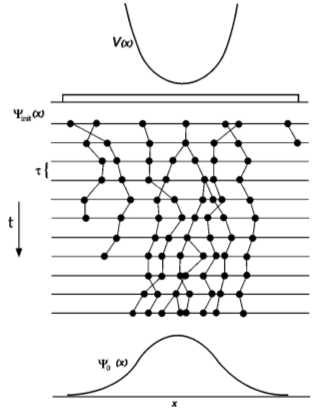
\includegraphics[width=0.9\textwidth]{branch_full.png}
\end{figure}
\end{column}
\begin{column}{0.7\textwidth}
   {\color{blue}{Figure:}} Reprinted from W.M.C. Foulkes et al. \textit{Rev. Mod. Phys.,} 73:33-83, 2001.
\end{column}
\end{columns}
\end{frame}

\begin{frame}{Diffusion Monte Carlo - Implementation}
\begin{enumerate}
   \item Start with N configurations (walkers) from VMC
   \item Loop over each walker and do the following
   \begin{enumerate}
      \setlength\itemsep{0.2em}
      \item Propose a move, $\R' = \R + \chi$, where $\chi$ is a vector of random numbers from the shifted Gaussian $\exp\left(\frac{m}{2\hbar^2\Delta\tau}\left(\R'-\R+2\frac{\nabla\Psi_I(\R')}{\Psi_I(\R')}\right)^2\right)$.
      \item The move is then accepted with the probability $A(\R'\leftarrow\R)=\mathrm{min}\left(1,\frac{\Psi_T^2(\R')}{\Psi_T^2(\R)}\right)$.
      \item Calculate the weight $w(\R')=\exp\left(-\left(E_L(\R')+E_L(\R)-2E_0\right)\Delta\tau/2\right)$.
      \item Do branching.
      \item Calculate and collect the observables and uncertainties needed and increase the imaginary time by $\Delta\tau$.
   \end{enumerate}
   \item Repeat from step 2 to 6 until the uncertainties are small enough.
\end{enumerate}
\end{frame}
\fi

\end{document}
